\chapter{\IfLanguageName{dutch}{Stand van zaken}{State of the art}}
\label{ch:stand-van-zaken}

% Tip: Begin elk hoofdstuk met een paragraaf inleiding die beschrijft hoe
% dit hoofdstuk past binnen het geheel van de bachelorproef. Geef in het
% bijzonder aan wat de link is met het vorige en volgende hoofdstuk.

% Pas na deze inleidende paragraaf komt de eerste sectiehoofding.


%---------- Objectherkenning -----------------------------------------------------------
\section{De werking van objectherkenning}\label{sec:ls-object-detectie}
Omdat objectdetectie de kern van de proof-of-concept zal vormen, is het van essentieel belang om eerst een grondig begrip te defini\"eren van wat deze techniek precies inhoudt.
In dit hoofdstuk zal eerst computer visie aan bod komen, een van de gebieden van hedendaagse artifici\"ele intelligentie, waarbinnen objectherkenning zich plaats vindt.
Dit zal verduidelijkt worden aan de hand van enkele praktische toepassingen die vandaag al in gebruik genomen worden met behulp van computer visie en objectherkenning.
Daarna volgt een uitleg van de processen waarop beelden opgeslagen en verwerkt worden ter voorbereiding op het toepassen van objectherkenning.
Tot slot worden enkele traditionele objectdetectie algoritmen besproken die de verwerkte data kunnen interpreteren.
Met een begrip voor de verschillende stappen van computer visie en objectherkenning kan vervolgens gekeken worden naar de volgende stap die toegepast zal worden in de proof-of-concept.
Het volgende hoofdstuk in deze literatuurstudie gaat hierop verder met meer informatie rond grote taalmodellen (LLM), een ander domein binnen kunstmatige intelligentie.

\subsection{Computer visie}\label{subsec:de-kern-van-objectdetectie}
Computer visie is een van de vele vakgebieden binnen de kunstmatige intelligentie en richt zich op het interpreteren van multimedia~\autocite{Moin2023}.
Met de komst van dit vakgebied ontstaat een grote waaier aan mogelijkheden voor computers om bij te staan bij complexere taken zoals gezichts- en emotieherkenning, sc\`eneanalyse en objectherkenning.
Hiermee beschrijven~\textcite{Tasnim2023} dat objectdetectie een fundamentele taak omvat binnen dit vakgebied waarmee het identificeren en lokaliseren van objecten mogelijk wordt op (bewegende) beelden.
De ontwikkelingen in dit vakgebied worden vandaag steeds meer gebruikt in allerlei sectoren:

\subsubsection{Computer visie in de landbouwsector}
\textcite{Radojcic2023}~beschrijft in zijn conferentiepaper voor de 15de Internationale Landbouwsymposium `AGROSYM 2023' conferentie het volgende over computer visie in de landbouw:
``De integratie van robotica, slimme landbouw en computervisietechnologie\"en in de landbouw heeft een transformerende verschuiving in de industrie teweeggebracht.
Het gebruik van computervisiealgoritmen heeft een cruciale rol gespeeld in het realtime monitoren en beheren van gewassen.
Door afbeeldingen en video's te analyseren, bieden deze algoritmen boeren tijdige en nauwkeurige informatie over de groei en ontwikkeling van hun gewassen, waardoor ze ge\"{\i}nformeerde beslissingen kunnen nemen over bemesting, irrigatie en pesticidegebruik.''
Deze resultaten binnen de landbouwsector worden gerealiseerd door middel van objectherkenning binnen computervisie.
Om het gebruik hiervan mogelijk te maken worden deep learning algoritmes zoals convolutionele neurale netwerken (CNN) toegepast, meer hiervan komt aan bod in het hoofdstuk~\nameref{sec:datasets}.

\subsubsection{Computer visie in zelfrijdende auto's}
Een tweede voorbeeld is het toepassen van computer visie in de transportsector.
Met behulp van computer visie-algoritmen zoals kleurenruimte transformatie, Canny-randdetectie en Hough-lijntransformatie wordt het mogelijk voor zelfrijdende auto's om op een goedkopere wijze berekeningen te maken~\autocite{Gajjar2023}.
Door middel van deze algoritmen verdwijnt de noodzaak om te ondersteunen op duurdere systemen, met name Lichtdetectie- en afstandmetingssensoren (LiDAR) die gebruikt worden om een virtuele driedimensionele map te maken van de direct omgeving.
Beide systemen kennen een vorm van objectherkenning om objecten zoals verkeersborden of voertuigen in de omgeving te detecteren.
De implementatie hiervan kent echter de moeilijkheid van data-analyse in donkere momenten zoals na zonsondergang, waardoor de kwaliteit van binnenkomende data afzwakt door het lage licht.
Een mogelijke oplossing hierbij is het toevoegen van infrarood lampen gecombineerd met een infraroodcamera.
Ook hierbij wordt het mogelijk om via CNN-algoritmes te bepalen wanneer overgestapt moet worden op een alternatief systeem.
\begin{figure}
    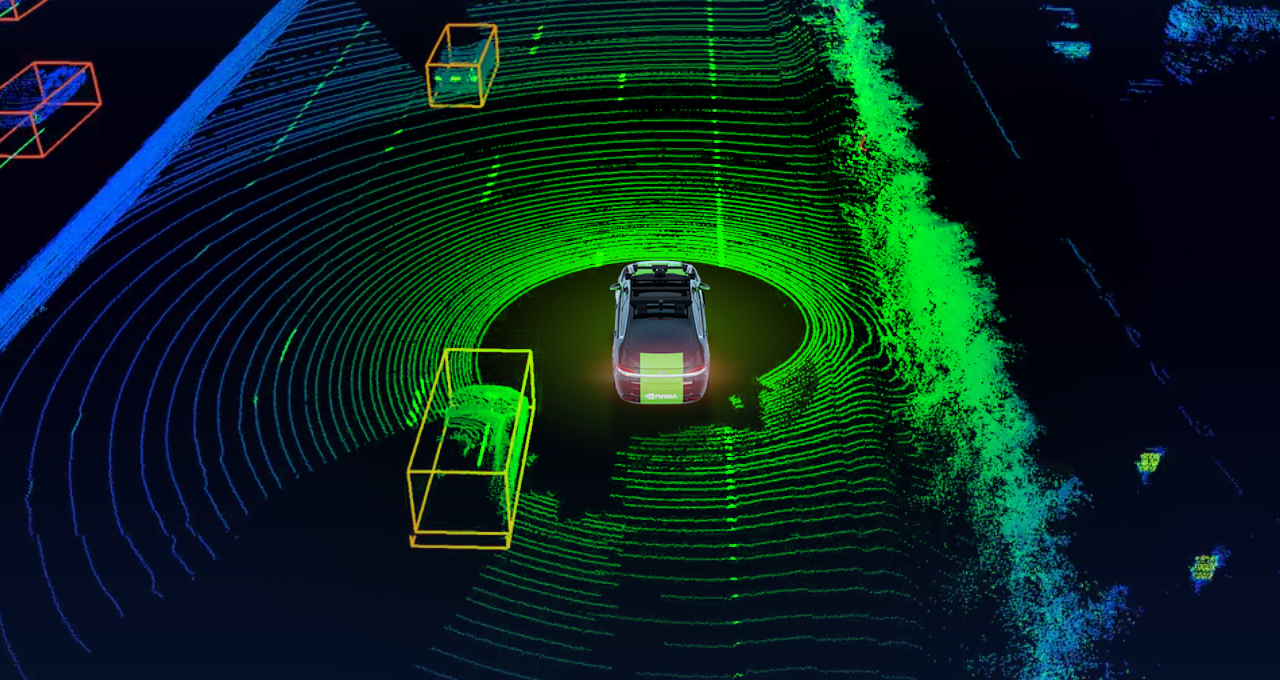
\includegraphics[width=1\linewidth]{images/visualisatie-lidar}
    \caption{Visualisatie van een LiDAR-systeem met objectherkenning in auto's~\autocite{Badoni2021}}
    \label{fig:visualisatie-lidar}
\end{figure}

\subsection{Beeldfragmenten in datavorm}\label{subsec:beeldfragmenten-als-data}
Concreet worden beelden digitaal opgeslagen in tweedimensionale tabellen van pixels, waarbij elke pixel kleurdata bevat.
De resolutie, of scherpheid, van een beeldfragment wordt vaak hierin uitgedrukt.
Zo kent een standaard Full HD (FHD)-computerscherm volgens de specificaties van~\textcite{VESA2013} een resolutie van 1920 pixels bij 1080 pixels.
Deze resolutie wordt volgens statistieken van~\textcite{ValveCorporation2024} gebruikt door meer dan de helft van haar gebruikers.
Om de kwaliteit van een beeldfragment uit te drukken wordt regelmatig gebruik gemaakt van de meeteenheid megapixels, waarbij \'e\'en megapixel \'e\'en miljoen pixels voorstelt.
Hiermee ontstaat de vaststelling dat de voorafgaande en meest gebruikte specificatie van Full HD een beeldkwaliteit van 2,1 megapixels kan weergeven aan gebruikers.

\subsubsection{Kwaliteit van hedendaags camera's}
Moderne smartphones zoals de Galaxy S24 nemen volgens~\textcite{Samsung2024} foto's aan een kwaliteit van 50 megapixels en bieden daarmee ongeveer 24 keer hogere kwaliteit dan een Full HD-computerscherm kan weergeven.
Het is hierbij belangrijk om op te merken dat het aantal megapixels niet de enige factor speelt in het bepalen van beeldkwaliteit.
Deze meeteenheid bepaalt tevens enkel de totale grootte van de data dat een beeldfragment bevat.
Ook ongewenste data, waaronder ruis en vervorming, worden hierin meegeteld.
Om dit probleem te mitigeren wordt in vele gevallen aan pixel binning gedaan, een proces waarbij pixels gegroepeerd worden tot zogenaamde superpixels~\autocite{Jin2012}.
\begin{figure}
    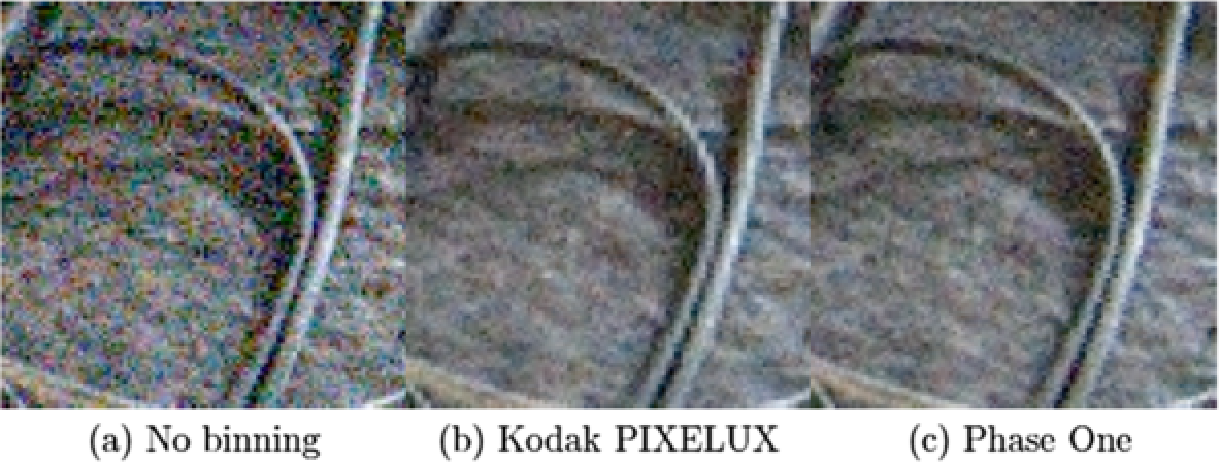
\includegraphics[width=1\linewidth]{images/pixel-binning}
    \caption{Visualisatie van pixel binning~\autocite{Jin2012}}
    \label{fig:pixel-binning}
\end{figure}
Moderne smartphones kiezen ervoor om pixels samen te nemen in groepen van vier en daarmee het binningsproces uit te voeren.
Ten gevolge van dit proces krijgen afbeeldingen een kleinere voetafdruk, wat resultaat in beelden van 12 megapixels.
Een bijkomend effect is het verzachten van observeerbare ruis waardoor beelden die genomen zijn in donkere plekken een hogere beeldkwaliteit krijgen.
De kwaliteit van beelden na het uitvoeren van dit proces liggen tussen die van de schermresoluties 4K Ultra HD (ongeveer 8 megapixels) en 8K Ultra HD (ongeveer 33 megapixels), resoluties die steeds vaker gebruikt worden in televisies~\autocite{Statista2024}.
Bovendien maakt dit het makkelijker voor computer visie-algoritmen om de gemaakte multimedia te analyseren aan een hogere nauwkeurigheid doordat er meer bruikbare data is om mee te werken.

\subsection{Het verwerken van data uit multimedia}\label{subsec:het-verwerken-van-data}
In hoofdstuk 2 van zijn onderzoek beschrijft~\textcite{Olaoye2024} het proces van beeldverwerking in enkele cruciale stappen:
% TODO: uitwerken
% beeldregistratie, filtering, segmentatie en kenmerkextractie.

\subsection{Bestaande objectherkenningsalgoritmen}\label{subsec:bestaande-algoritmen}
Na het verwerken van beeldfragmenten komt het toepassen van objectherkenning aan bod, waarvoor vele iteraties aan algoritmes geschreven zijn.
Belangrijk hierbij is om te onthouden dat elk algoritme eerst een dataset nodig heeft om te weten hoe een bepaald object eruit ziet.
Dit komt aan bod in het hoofdstuk~\nameref{sec:datasets}.
Hieronder volgen de meestgebruikte traditionele algoritmes om aan objectherkenning te doen.
Daarnaast worden enkele actuele toepassingen opgesomd en de effici\"entie van de algoritmes.

% TODO: algoritmes
\subsubsection{Algoritme A}
Algoritme A wordt uitgelegd.

% TODO: uitdagingen en beperkingen van objectdetectie
% variaties in verlichting, complexe achtergronden, schaalvariaties, vervormingen en occlusie.


%---------- De werking van AI ----------------------------------------------------------
\section{De werking van grote taalmodellen}
\label{sec:ls-artificiele-intelligentie}
In het vorig hoofdstuk kwam computer visie aan bod als vakdomein binnen de artifici\"ele intelligentie.
Een ander, en met hedendaagse coverage in het nieuws wellicht bekendere, domein hierin is de toepassing van large language models (LLM).
Voorbeelden hiervan zijn GPT en haar toepassing ChatGPT. % TODO: hier op verder gaan & kijken naar voorstel of daar niets uit genomen kan worden.

%---------- Datasets generereren ------------------------------------------------------
\section{Het trainen van datasets voor objectherkenning}\label{sec:datasets}
Uitleg hier over: % TODO
- hoe wordt bepaald wat een geldig beeld is om mee te trainen
- hoe worden datasets getraind
- misschien statistieken van hoe nauwkeurig
- bestaande datasets gebruiken zoals Google Gemini Vertex
%  populaire datasets, zoals COCO (Common Objects in Context), Pascal VOC (Visual Object Classes), en ImageNet, worden vaak gebruikt voor het trainen en evalueren van objectherkenningsalgoritmen.